\newcommand{\invariantpanel}[3]{%
\begin{figure}[H]\centering
\includegraphics[page=#1,width=\linewidth]{figures/forms-by-invariant.pdf}
\caption{#2. Each row reports raw unique ASTs, v3.3 structural forms and v3.3 fixed-command components for that invariant, in that order. Bar lengths share a scale
within each problem; the numbers give the exact counts.}\label{#3}
\end{figure}}
\invariantpanel{1}{Unique forms by invariant: classroom, courses, and CV}{fig:scoped-by-invariant}
\invariantpanel{2}{Unique forms by invariant: graphs, LTS, production lines, and social media}{fig:scoped-by-invariant-middle}
\invariantpanel{3}{Unique forms by invariant: train stations and trash}{fig:scoped-by-invariant-last}
